\section{NLP Aspects Overview}
\par
As stated in the introduction section the goal of project becomes that of identifying the arguments and the relations that exist between them in a given text. As such, the task of this module can be modeled as a classification problem.
\par
As presented previously, there exist a number of models for both the intrinsic structure of a model, as well as for the relations that can hold between them.
The above sections gave a classification of the different types of dialog and argumentation schemes. What is interesting to notice is that each type of dialog supports some argumentation schemes better than others. Thus, having chosen one specific type of dialog, the most relevant argumentation schemes pertaining to that dialog model will be chosen as structure guidelines for our arguments. 
In addition, a Toulmin (S. E. Toulmin. \textit{The Uses of Argument}) based alternative representation of an argument will be considered.

\subsection{Main problems}
\par
Having laid out this model, we are faced with the following challenges of Argumentation Mining: 
\begin{description}
\item Detect all the arguments in a free text (classification problem)
\item Determine argument limits ( segmentation problem)
\item Determine arguments type (complex)
\item Detect argumentation structure (complex)
\end{description}
\par
The Corpus that will be used to for solving the above problems is the one provided by \textit{Arauacaria} (\textit {http://www.arg.dundee.ac.uk/projects/araucariadb/search.php}), which, albeit being not very large, has the advantage of giving annotated argument examples.
\par
In the work by R.M. Palau and M-F Moens\cite{palau1} some solutions to this problems are proposed, some of which we consider to be very useful for our project. For the problem of argument detection statistical classifiers are employed. In particular, good results can be obtained by using the \textit{maximum entropy model} and \textit{multinomial naive Bayes} classifier which learns a model of the joint probability of an element \textit{x} and its label \textit{y}, \textit{p(x, y)}, and makes its predictions by using Bayes rule to calculate p(y\textbar x) and then selects the most likely label \textit{y}.
\par
For the problem of determining argument limits (grouping of argumentative statements into their corresponding argument) we consider computing the semantic distance between different argumentative units (sentences) and group sentences in one argument if they discuss content that is semantically related. Like in the work of Palau and Moens, we assume that the relatedness of two sentences is a function of the relatedness of their words. We want to employ an ontology based semantic relatedness measure, where the relatedness of words depends on their semantic distances in a lexico-semantic resource such as WordNet.
\par
In the determination of argument types, we also consider the use of statistical classifiers.
The problem here is that while a classification of argumentative statements into premises and conclusions is possible (as shown by Palau and Moens by use of a SVM), the task of determining a specific scheme for an argument is much more challenging. In particular, we have to rely on some domain ontology in order to be able to find semantic features that will allow us to classify the arguments as belonging to a certain scheme.
\par
Extensive use of other NLP tools such as POS taggers will also be made in order to enrich the possible set of features used for classification.
\par
Lastly, the problem of determining the argumentation structure, that is, of relations existing between the arguments, will have to take all the results obtained by the previous steps into consideration. The employed algorithm will make the assumption that the discourse follows the rules of the chosen dialog type and that arguments used within it belong to the appropriate argumentation schemes.

\section{Natural Language Module architecture}
\par
This section gives a general overview of the most important modules of our application. We will give a graphical representation of the main modules and of the relation between them. Afterwards, we will give a more detailed description of each module, highlighting the approaches and algorithms considered for their implementation.

\begin{center}
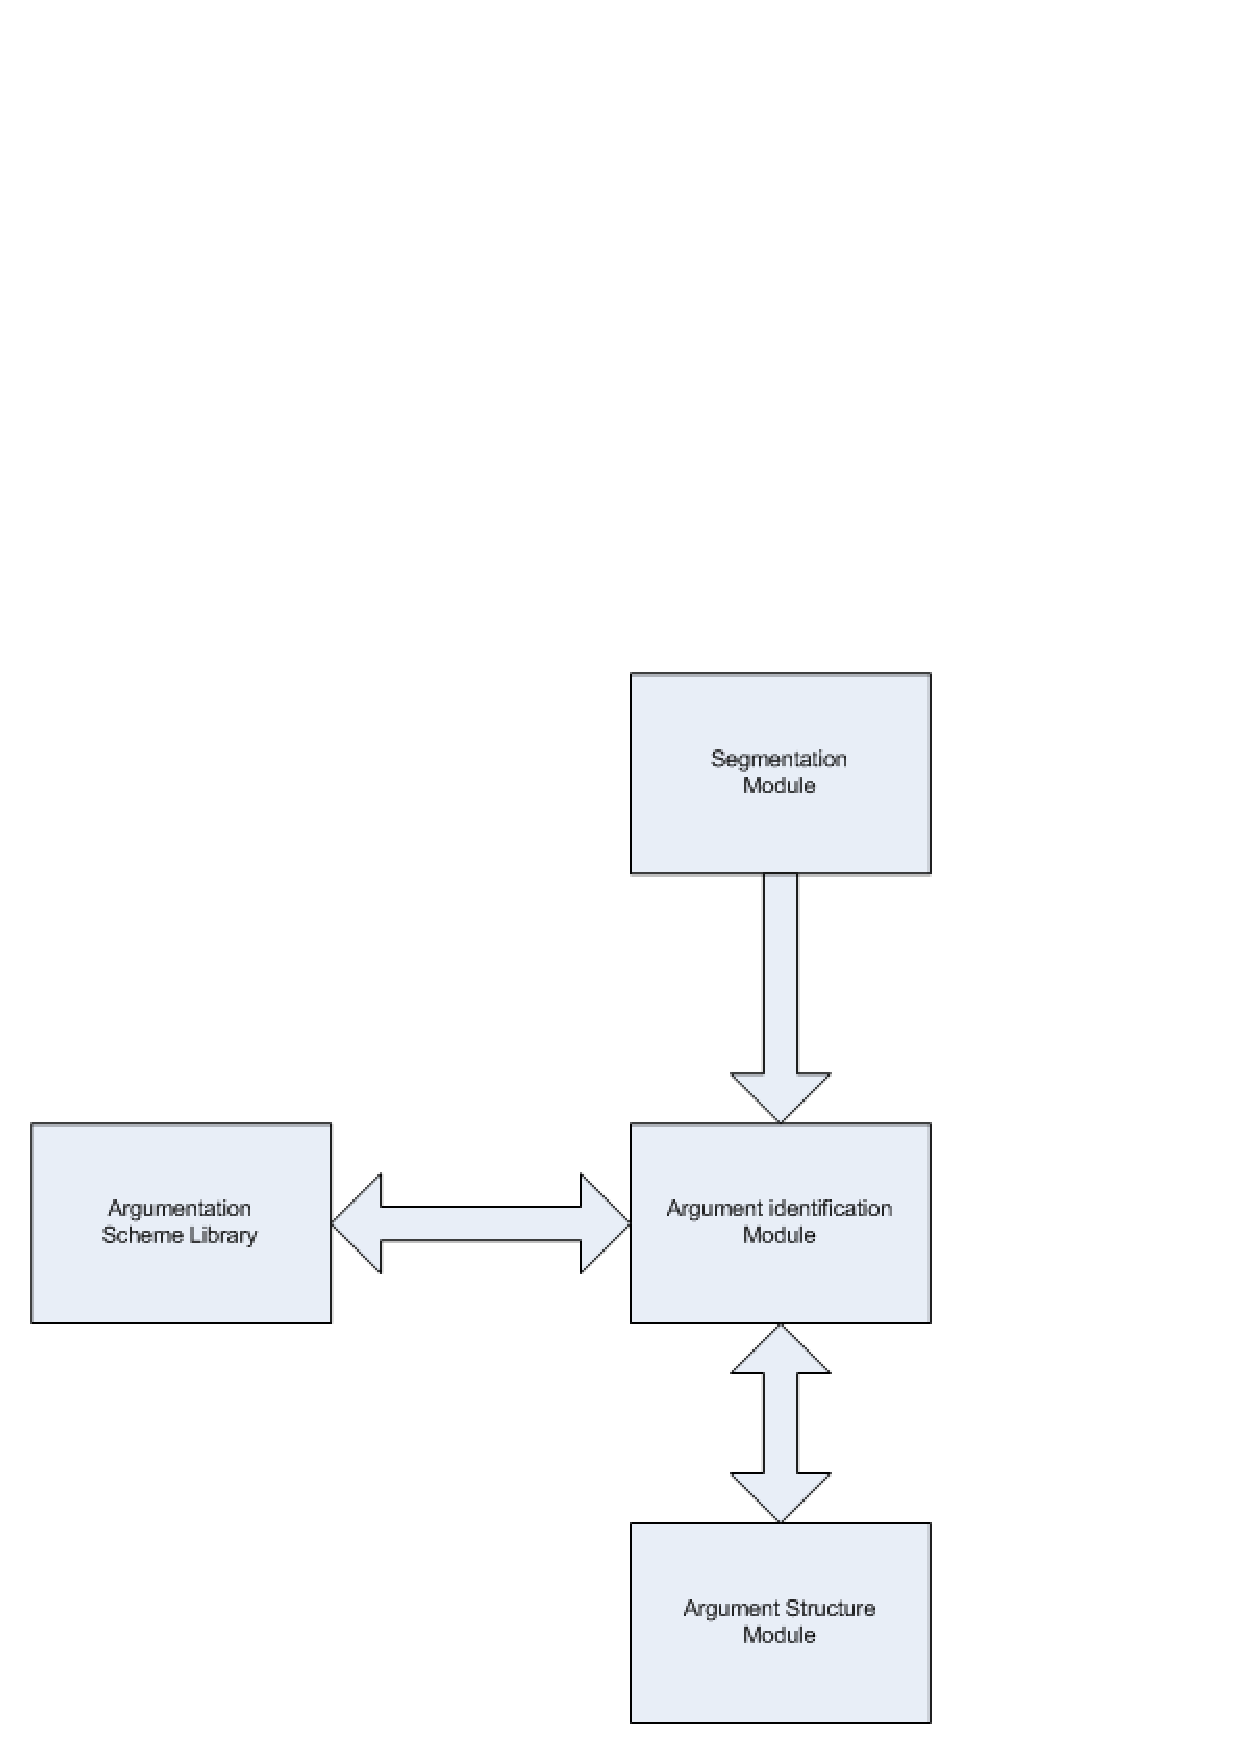
\includegraphics{NLP_Architecture.png}
\end{center}

\subsection{Argumentation Identification Module}
\par
The Segmentation Module classifies all sentences into argumentative and non-argumentative utterances. This module's essential role is to determine which parts of the text are also part of arguments.
\par
The main assumption used by this module is that various arguments are made up from smaller units called elementary units. An elementary unit represents a span of text that can't be further divided from an argumentation point of view. We use sentences as elementary units because naturally people structure their ideas in sentences. There are some cases in which only a part of a sentence is part of an argument and the rest of the sentence has no argumentative function. In this case we will include the entire sentence in the argumentation analysis.
\par
We have used two classifiers from the Natural Language Toolkit(NLTK)\label{NLTK} library: the naive Bayesian classifier and the maximum entropy classifier. For both classifiers we have used the same set of features:
\begin{description}
\item[Adverbs] Detected with a part-of-speech (POS) tagger from NLTK.
\item[Verbs] Detected with a POS tagger. Only the main verbs (excluding ``to be'', ``to do'' and ``to have'') are considered.
\item[Modal auxiliary] Indicates if a modal auxiliary is present using a POS tagger.
\item[Text statistics] Sentence length, average word length and number of punctuation marks.
\item[Punctuation] The sequence of punctuation marks present in the sentence is used as a feature (e.g. ``:.''). When a punctuation mark occurs more than once in a row, it is considered the same pattern (e.g. two or more successive commas both result in ``,+'').
\item[Key words] Keywords refer to several words or word sequences obtained from a list of terms indicative for argumentation. Examples from the list are ``but'', ``consequently'', and ``because of''.
\end{description}
\par
In building these features we have used the Punkt Word Tokenizer and the Punkt Sentence Tokenizer from NLTK. This splits the text into sentences quite well but it's not one hundred percent accurate. In addition to this Araucaria is annotated by humans and in several cases the assumption we made on the argument delimitation is violated. Because of this we use an algorithm that matches intervals of sentences from training examples with those obtained from parsing.
\par
From the above mentioned features only the presence of key words specific to argumentation is computationally expensive using a classical approach. Instead of comparing each word with every word in a list we have used the Aho-Corasick algorithm that has a running time linear in the size of the text plus the total number of matches.
\subsection{Segmentation Module}
\par
The Argumentation Identification Module uses this module to partition different argumentative sentences (units) into their corresponding arguments, that is, to determine the limits of each individual argument.
\par
In order to achieve this we opt to calculate the semantic distance between the different argumentative units, and group sentences in one argument if they discuss content that is semantically related. As in the work of Palau and Moens, we assume that the relatedness of two sentences is a function of the relatedness of their words.
\par
Given this assumption we take the semantic relatedness of words to be given by their semantic distances in a lexico-semantic resource such as WordNet.
\par
Measures of relatedness are more general in that they can be made across part of speech boundaries, and they are not limited to considering is-a relations.
\par
Several measures of relatedness which are based on the WordNet database can be used.
\begin{itemize}
\item The hso (Hirst and St-Onge, 1998) measures classifies relations in WordNet as having direction, and then establishes the relatedness between two concepts A and B by finding a path that is neither too long nor that changes direction too often. 
\item The lesk (Banerjee and Pedersen, 2003) and vector measures incorporate information from WordNet glosses. The lesk measure finds overlaps between the glosses of concepts A and B, as well as concepts that are directly linked to A and B. 
\item The vector measure (Patwardhan, 2003) creates a co-occurrence matrix for each word used in the WordNet glosses from a given corpus, and then represents each gloss/concept with a vector that is the average of these co-occurrence vectors.
\end{itemize}
\par
WordNet provides modules that implement these measures and that offer a specific API for their usage.
\par
Using these measures we can compute an overall semantic relatedness of the argumentation units. By means of a clustering algorithm that will use the distances given by the above mentioned methods we can then segment sentences into their corresponding arguments (clusters), thus finding the intended argument limits.
\par
We assume the semantic relatedness of words to be given by their semantic distances in a lexico-semantic resource such as WordNet. We use the lin similarity measure to compute the relatedness of two synsets. As each word in a sentence can have several senses, one would first have to go through a word sense disambiguation process to determine the most probable meaning. As this process is time-consuming, the current approach employs the use of the most common sense, as defined by WordNet, for each word we encounter.
\par
Using the lin\cite{lin} similarity we compute a word similarity matrix between every pair of words, one from each sentence.To compute the estimated similarity between two sentences we then use the following method. Given two sentences A and B, for each word from sentence A we compute the most similar word from sentence B, as given by the previously computed matrix.

\[ b^* = arg \max_b Sim(a,b) \]

\paragraph*{In a similar manner, for each word in sentence B we compute the most similar word from sentence A.}

\[ a^* = arg \max_a Sim(a,b) \]

\par
Afterwards the similarity between sentences A and B is given by

\[ ( \sum{a^*} + \sum{b^*}) / (2 * (\mid A\mid + \mid B \mid ) \]

\par
The above process yields a sentence similarity matrix. This matrix is used as an input to a hierarchical clustering algorithm. We take an empirically determined cutoff distance of 0.875 to cut the resulting cluster dendrogram at the corresponding depth. This results in a list of sentence clusters, each of which contains the components of an individual argument.

\subsection {Argumentation Scheme Library}
\par
The Argumentation Scheme Library contains abstract forms of argument that capture patterns of reasoning. Each argumentation scheme describes the relations between internal parts (the premises and the conclusion) of a complex argument and, also, the set of critical questions that may attack that argument. Chris Reed and Douglas Walton, in their research report ``Towards a Formal and Implemented Model of Argumentation Schemes in Agent Communication''\cite{reed} describe the conventional techniques to handle the structure of argumentation schemes in such way that agents may use them in reasoning and also that communication structures can be built around those schemes.
\par
An example of Argumentation Scheme is Argument from Position To Know:
\begin{description}
\item[Major Premise]: Source \emph{a} is in a position to know about things in a certain subject domain \emph{S} containing proposition \emph{A}.
\item[Minor Premise]: \emph{a} asserts that \emph{A} (in Domain \emph{S}) is true (false).
\item[Conclusion]: \emph{A} is true (false).
\end{description}
This type of argument is defeasible by questioning. Matching the argument from position to know are three critical questions:
\begin{description}
\item[CQ1]: Is \emph{a} in a position to know whether \emph{A} is true (false)?
\item[CQ2]: Is \emph{a} an honest (trustworthy, reliable) source?
\item[CQ3]: Did \emph{a} assert that \emph{A} is true (false)?
\end{description}
\par
Our Argumentation Scheme Library will be trained from Araucaria DB, which contains several real instantiations of argumentation schemes. For representation Argument Markup Language(AML)\label{AML} is used, which in turn is based upon the industry standard XML.
\par
The scheme library contains some abstract schema from the Walton schema set\cite{reed}. These are used in turn for mapping the actual discourse and creating schema instantiations. Thus an argumentation is represented as the relation between arguments as elementary units and the type of relation is given by a schema. In\cite{reed} each schema has an unique name and we have used the same names as they describe the schema.

\subsection{Argument Structure Module}
\par
The Argument Identification Module and Segmentation Module were used to distinguish between argumentative and non-argumentative sentences and to group argumentative sentences together into their corresponding argument.
\par
The purpose of this module thus becomes to determine the internal structure of an argument, i.e. the organization of its clauses into conclusions and supporting premises and to group arguments into argumentation structures by instantiating schemas from the Schema Library.
\par
This relies again on work done by Palau and Moens in \cite{palau1} and \cite{palau2} and considers the partition of an argument's units into premises or conclusions. For each argument, certain features will be determined. The list can comprise features such as:
\begin{description}
\item[Tense of Main Verb]: Tense of the verb from the main clause of the sentence; having as nominal values ``Present'', ``Past'' or ``No Verb''.
\item[History]: The most probable argumentative category of previous and next sentence.
\item[Rhetorical Patterns]: Type of rhetorical pattern occurring on current, previous and next sentences (e.g. ``however,'')
\item[Argumentative Patterns]: Type of argumentative pattern occurring in sentence
\end{description}
A SVM (Support Vector Machine) based algorithm that uses these features will then be used to classify the sentences of an argument into either premises or conclusions.
\par
In addition to just distinguishing between premise and conclusion, this approach tries to map the argument's structure onto one or several argumentation schemes. 
The definition and format of these schemes is provided by the Argumentation Scheme Library module. 
\par
For this task we tried a SVM based on various features and a HMM based on the number of arguments and identification of main subject and relevant noun phrases.

\section{NLP Module Results}
\par
We have trained the NLP module on Araucaria corpus. This is an mixed corpus and albeit small it provides a good measure of argumentation in various domains. This section outlines some of the results obtained with this module.

\subsection{Argument Identification Module}
The Araucaria corpus, consisting of approximately one thousand AML files was split in half for training and testing of both classifiers. At sentence level the Punkt module has an accuracy around 90\% and the reader may refer to \cite{kiss} for details about the algorithm used by this tokenizer.
\par
For the problem of classification of sentences as argumentative or non-argumentative both the naive Bayesian and the maximum entropy gave approximately the same results. Overall the maximum entropy is slightly better with an average difference in accuracy of 2\%. We obtained around 78\% accuracy with a recall around 85\%. In their work \cite{palau1} Palau and Moens obtained a better accuracy using HUDOC corpus.

\begin{figure}[tbh]
\centering
\includegraphics[scale=0.6]{accuracy.jpg}
\caption{Accuracy for Naive Bayesian Classifier}
\label{fig:acc}
\end{figure}

As we can see in figure \ref{fig:acc} there is a good performance overall but there are cases in which the accuracy is as low as 20\%. This can be explained by the structure of Araucaria. Because it is an argumentation corpora the number of argumentative sentences is much larger than the number of non-argumentative ones. There are AML files that do not fall into this general pattern and the classifiers gives poor results for this instances.

\begin{figure}[tbh]
\centering
\includegraphics[scale=0.59]{f1score.jpg}
\caption{F1 score for the maximum entropy classifier}
\label{fig:f1s}
\end{figure}
\par
In figure \ref{fig:f1s} the F1 score is shown for a session of testing of the maximum entropy classifier. This shows an overall good performance of the classifier.

\begin{figure}[tbh]
\centering
\includegraphics[scale=0.9]{recall.jpg}
\caption{Plot of the recall for the maximum entropy classifier}
\label{fig:rec}
\end{figure}

\par
As shown in figure \ref{fig:rec} the maximum entropy classifier has a good recall and because we want argumentative sentences this is a good measure of performance. Even if some of the non-argumentative sentences are classified as argumentative they will be part of some argument in the segmentation phase and won't alter the result.
\par
As shown above the classification of sentences in argumentative and non-argumentative is a feasible problem and we have obtained good results on Araucaria corpus. However in a multi agent argumentation system usually the arguments exchanged with humans tend to have a better structure, imposed by the form of communication. This argumentation is based on dialog and we humans tend to give one argument at time or at most a small argumentation structure to support an argument and then wait for a reply.
\par
From the point of view of classification this is very different from texts, in which an entire argumentation is given in the text in addition to non-argumentative spans of text that may interleave with it. Because of this we have tested the argument identification module on several dialog based argumentation texts produced by us and our colleagues in the Natural Language Processing course. Although the number of tests is relatively small we have noticed a slight increase in accuracy that proves the system is suited usage in a dialog based multi agent system.

\subsection{Segmentation Module}  
\par
The role of the segmentation module is that to partition different argumentative sentences (units) into their corresponding arguments, that is, to determine the limits of each individual argument.
\par
As presented in the description of the NLP module capabilities, we opt to calculate the semantic distance between the different argumentative units, and group sentences in one argument if they discuss content that is semantically related.
\par
The module receives a list of argumentative sentences as its input. It then uses a word tokenizer to split the sentences into lists of words. Stopwords such as "the", "in", "with" etc. are removed before going to the next step.
\par
Here is a simple example. The initial text:
\paragraph*{\emph{``It is well established that if any statement is made on the floor of the House by a Member or Minister which another Member believes to be untrue, incomplete or incorrect, it does not constitute a breach of privilege.  In order to constitute a breach of privilege or contempt of the House, it has to be proved that the statement was not only wrong or misleading but it was made deliberately to mislead the House.  A breach of privilege can arise only when the Member or the Minister makes a false statement or an incorrect statement willfully, deliberately and knowingly.    On a perusal of the comments of the Ministers in the matter, I am satisfied that there has been no misleading of the House by them as alleged by the Member.   I have accordingly disallowed the notice of question of privilege.  Copies of the comments of the Ministers have already been made available to Dr. Raghuvansh Prasad Singh.''}}
\paragraph*{The determined word lists:}
\begin{description}
\item[L1:][`It`, `well`, `established`, `statement`, `made`, `floor`, `House`, `Member`, `Minister`, `another`, `Member`, `believes`, `untrue`, `incomplete`, `incorrect`, `constitute`, `breach`, `privilege`]
\item[L2:] [`In`, `order`, `constitute`, breach`, `privilege`, `contempt`, `House`, `proved`, `statement`, `wrong`, `misleading`, `made`, `deliberately`, `mislead`, `House`]
\item[L3:] [`A`, `breach`, `privilege`, `arise`, `Member`, `Minister`, `makes`, `false`, `statement`, `incorrect, `statement`, `wilfully`, `deliberately`, `knowingly`]
\item[L4:] [`On`, `perusal`, `comments`, `Ministers`, `matter`, `I`, `satisfied`, `misleading`, `House`, `alleged`, `Member`]
\item[L5:] [`I`, `accordingly`, `disallowed`, `notice`, `question`, `privilege`]
\item[L6:] [`Copies`, `comments`, `Ministers`, `already`, `made`, `available`, `Dr`, `Raghuvansh`, `Prasad`, `Singh`]
\end{description}
\par
The (symmetric) sentence similarity matrix:
\begin{center}
  \begin{tabular}{ | l | c | c | c | c | c | c | }
    \hline
	& \emph{1} & \emph{2} & \emph{3} & \emph{4} & \emph{5} & \emph{6} \\ \hline
    \emph{1} & 1.00 & 0.24 & 0.24 & 0.19 & 0.10 & 0.13  \\ \hline
	\emph{2} & 0.24 & 1.00 & 0.21 & 0.19 & 0.14 & 0.10  \\ \hline
	\emph{3} & 0.24 & 0.21 & 1.00 & 0.16 & 0.13 & 0.11  \\ \hline
	\emph{4} & 0.19 & 0.19 & 0.16 & 1.00 & 0.13 & 0.12  \\ \hline
	\emph{5} & 0.10 & 0.14 & 0.13 & 0.13 & 1.00 & 0.06  \\ \hline
	\emph{6} & 0.13 & 0.10 & 0.11 & 0.12 & 0.06 & 1.00  \\ \hline
  \end{tabular}
\end{center}
\par
The resulting sentence clustering (only the indexes of the sentences are show):
\[ [[5], [4, 3, 1, 0, 2]] \]
\par
We can see that sentences 1-5 belong to one argument and sentence 6, which is actually non-argumentative, this being only an illustrative example, belongs to a separate cluster.
\par
The current method yields some promising results, but there is still room for improvement, especially in the process of determining word similarities, where we hope to be able to implement a more advanced measurement solution. In particular, the Lin measure can only compute the similarity between words which have the same part of speech (noun, verb etc). The lesk or gloss-vector measures, which we will try to implement in future developments can cross these boundaries and are not limited by is-a relations.

\subsection{Argument Structure Module}
\par
For the task of classification of sentences in premises and conclusions we have used cross validation with 7 bins to obtain a good measure of the performance of this module. Our SVM based algorithm uses the list of argumentative sentences partitioned in arguments as well as the list of non-argumentative sentences as history feature. We have obtained around 67\% accuracy for the SVM classifier.
\paragraph*{An example of the output of this classifier is shown below:}
\begin{description}
\item [[(To scientific naturalist this suggestion is "creationist" and therefore unacceptable in principle, because it invokes an entity unknown to science.', 1.0)], [(In that case there could be real prophets-persons with a genuine knowledge of God who are neither frauds nor dreamers.', 0.0), (Such persons could conceivably be dangerous rivals for the scientists as cultural authorities.', 1.0)], [(Suppose that a skeptic argues that evidence for biological creation by natural selection is obviously lacking, and that in the circumstances we ought to give serious consideration to the possibility that the development of life required some input from a pre-existing, purposeful creator.', 1.0), (What is worse, it suggests the possibility that this creator may have communicated in some way with humans.', 1.0)]]
\end{description}
\par
For determining the argumentation structure the results obtained so far are below average. The HMM proved a better choice but there is still a lot of space for improvements.
